\section{Allocation et évaluation historique}
\label{sec:allocation_backtest}

Un système de recommandation de portefeuille se juge, en dernier ressort, sur la performance des portefeuilles qu'il aurait recommandés. Cette section simule ces recommandations sur la période de test, avec un protocole qui interdit toute information future, et les compare à des stratégies simples de même risque.

\subsection{Protocole \emph{walk-forward}}

\begin{itemize}
  \item \textbf{Rebalancement mensuel}, le dernier jour de bourse de chaque mois, de janvier 2022 à novembre 2026 (60 rebalancements).
  \item À chaque date, la covariance est estimée sur les 252 jours précédents, et le régime avec les seules données disponibles.
  \item Entre deux rebalancements, les poids dérivent avec les prix ; les \textbf{coûts de transaction} (10 points de base par unité échangée) sont déduits à chaque rebalancement.
  \item Deux réglages ne sont appris par aucun modèle : la pénalité de rotation $\gamma$ et l'intensité de la réduction du risque en régime de stress. Ils sont choisis \textbf{sur la validation 2020-2021}, jamais sur le test.
\end{itemize}

\paragraph{Réglages choisis sur la validation.} Nous avons testé $\gamma \in \{0{,}5 ; 2 ; 5 ; 10\}$ et quatre intensités de réduction du risque en régime de stress (cible de volatilité multipliée par 1 ; 0,9 ; 0,75 ou 0,6), avec pour critère le ratio de Sharpe moyen des trois profils sur 2020-2021. Le choix retenu est $\gamma = 0{,}5$ et \textbf{aucune réduction}. Ce second résultat confirme la section~\ref{sec:regime_alerte} : les régimes de stress étant souvent suivis de rebonds, réduire le risque à ce moment fait vendre au mauvais moment. Le système garde l'agent Régime pour informer le client, mais ne s'en sert pas pour modifier l'allocation. C'est une décision guidée par les données, même si elle contredit l'intuition de départ.

\paragraph{Stratégies comparées.} Pour chaque profil, le système multi-agent est comparé à quatre références de risque comparable : son allocation stratégique de référence rebalancée chaque mois (sans optimisation) ; le 1/N, la parité de risque et HRP, chacun ramené à la volatilité cible du profil par un mélange avec la poche monétaire. Quatre références classiques complètent le tableau : 1/N brut, 60/40, variance minimale et Markowitz sur rendements historiques. Une limite doit être signalée : sans emprunt, on peut seulement \emph{réduire} le risque d'un portefeuille en ajoutant du monétaire. La parité de risque et HRP, naturellement peu risquées, restent donc en dessous des cibles des profils Équilibré et Dynamique ; pour ces profils, la comparaison porte sur le ratio de Sharpe plutôt que sur le rendement.

\subsection{Performances sur le test}

\begin{table}[!htb]
  \centering
  \small
  \caption{Performances sur le test (janvier 2022 à novembre 2026), nettes de coûts. Sharpe : rendement excédentaire au taux sans risque divisé par la volatilité. Rotation : somme des poids échangés par an.}
  \label{tab:backtest}
  \setlength{\tabcolsep}{5pt}
  \begin{tabular}{@{}l l r r r r r@{}}
    \toprule
    \textbf{Profil} & \textbf{Stratégie} & \textbf{Rendement} & \textbf{Volatilité} & \textbf{Sharpe} & \textbf{Perte max.} & \textbf{Rotation} \\
    \midrule
    \multirow{5}{*}{Prudent} & \textbf{Multi-agent} & \textbf{2,2 \%} & \textbf{6,3 \%} & $\boldsymbol{-0{,}26}$ & $\boldsymbol{-15{,}0}$ \textbf{\%} & \textbf{93 \%} \\
     & Référence stratégique & 3,2 \% & 7,4 \% & $-0{,}08$ & $-16{,}1$ \% & 46 \% \\
     & 1/N vol. cible & 4,8 \% & 6,9 \% & 0,13 & $-12{,}9$ \% & 81 \% \\
     & Parité de risque vol. cible & 4,1 \% & 6,6 \% & 0,04 & $-14{,}1$ \% & 90 \% \\
     & HRP vol. cible & 2,9 \% & 4,5 \% & $-0{,}23$ & $-11{,}1$ \% & 190 \% \\
    \midrule
    \multirow{5}{*}{Équilibré} & \textbf{Multi-agent} & \textbf{4,7 \%} & \textbf{9,6 \%} & \textbf{0,12} & $\boldsymbol{-18{,}2}$ \textbf{\%} & \textbf{74 \%} \\
     & Référence stratégique & 5,4 \% & 10,5 \% & 0,17 & $-18{,}6$ \% & 52 \% \\
     & 1/N vol. cible & 6,2 \% & 10,5 \% & 0,25 & $-18{,}0$ \% & 95 \% \\
     & Parité de risque vol. cible & 4,9 \% & 7,4 \% & 0,14 & $-15{,}1$ \% & 71 \% \\
     & HRP vol. cible & 2,8 \% & 4,6 \% & $-0{,}24$ & $-11{,}1$ \% & 194 \% \\
    \midrule
    \multirow{5}{*}{Dynamique} & \textbf{Multi-agent} & \textbf{8,1 \%} & \textbf{13,3 \%} & \textbf{0,35} & $\boldsymbol{-19{,}9}$ \textbf{\%} & \textbf{67 \%} \\
     & Référence stratégique & 8,3 \% & 13,7 \% & 0,36 & $-19{,}9$ \% & 58 \% \\
     & 1/N vol. cible & 7,1 \% & 11,7 \% & 0,30 & $-19{,}6$ \% & 61 \% \\
     & Parité de risque vol. cible & 4,9 \% & 7,4 \% & 0,14 & $-15{,}1$ \% & 70 \% \\
     & HRP vol. cible & 2,8 \% & 4,6 \% & $-0{,}24$ & $-11{,}1$ \% & 194 \% \\
    \midrule
    \multirow{4}{*}{--} & 1/N brut & 7,1 \% & 11,7 \% & 0,31 & $-19{,}6$ \% & 60 \% \\
     & 60/40 & 5,1 \% & 11,2 \% & 0,15 & $-20{,}9$ \% & 39 \% \\
     & Variance minimale & 1,3 \% & 4,9 \% & $-0{,}53$ & $-13{,}7$ \% & 111 \% \\
     & Markowitz historique & 17,0 \% & 19,5 \% & 0,70 & $-23{,}2$ \% & 616 \% \\
    \bottomrule
  \end{tabular}
\end{table}

\begin{figure}[!htb]
  \centering
  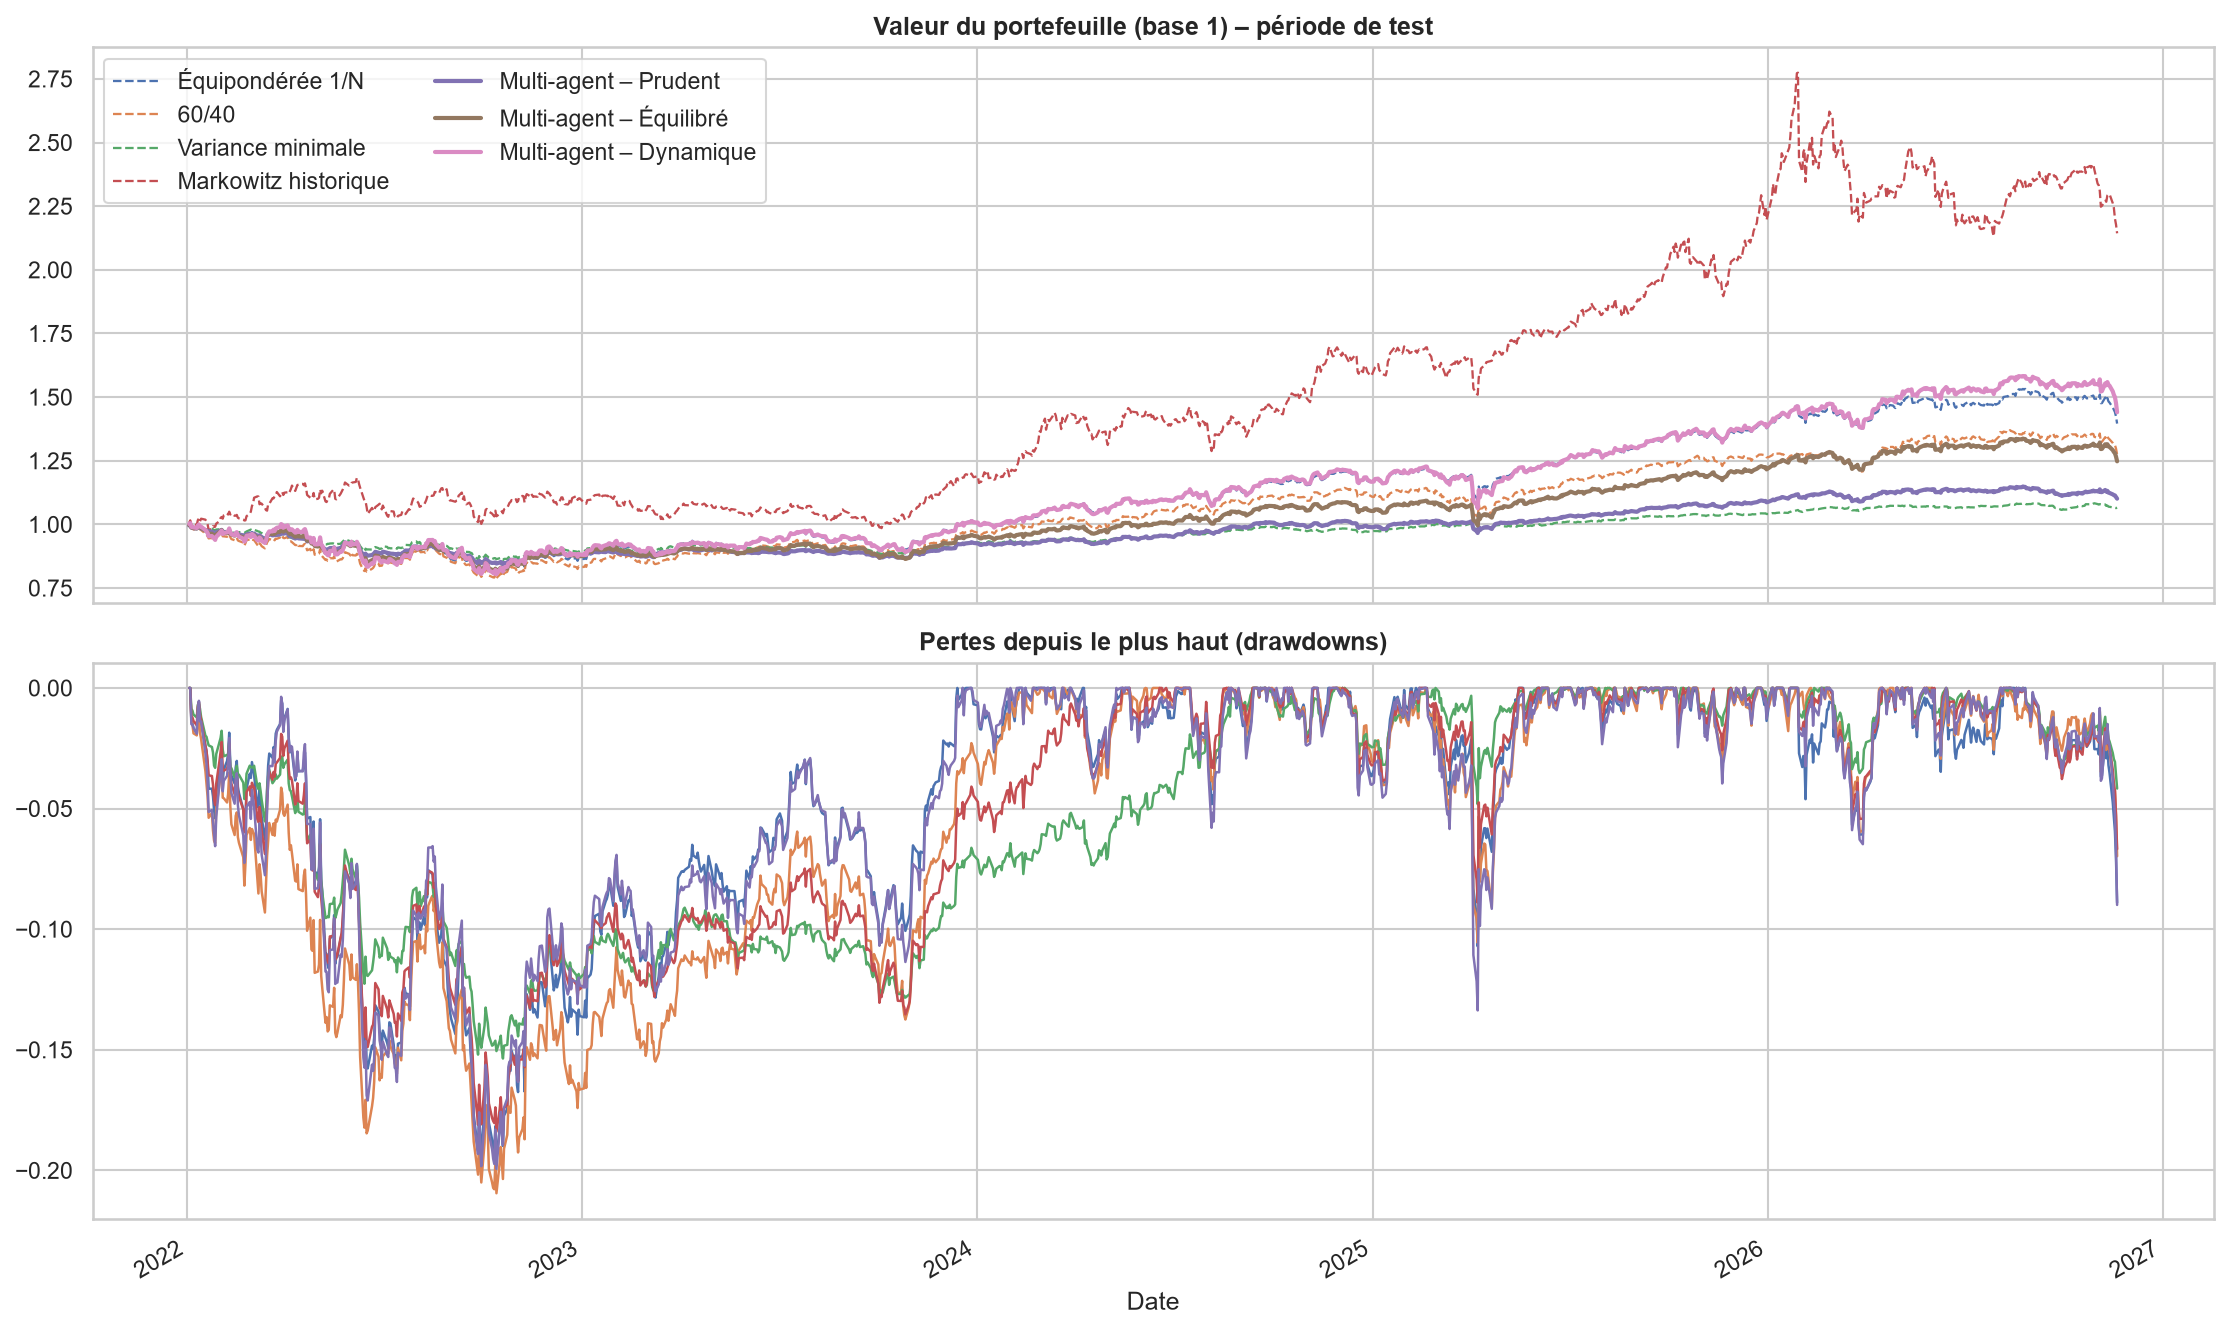
\includegraphics[width=\textwidth]{18_backtest_valeur_drawdown.png}
  \caption{Valeur des portefeuilles (base 1) et pertes depuis le plus haut sur la période de test.}
  \label{fig:backtest}
\end{figure}

\subsection{Significativité : bootstrap par blocs}

Sur moins de cinq ans, les écarts de ratio de Sharpe sont très bruités. Nous estimons un intervalle de confiance à 95 \% de la \emph{différence} de Sharpe entre le système et chaque référence par \textbf{bootstrap par blocs}~\cite{kunsch1989} : on rééchantillonne des blocs de 21 jours consécutifs, ce qui préserve l'autocorrélation et le regroupement de volatilité que détruirait un bootstrap ordinaire. Si l'intervalle contient zéro, la différence n'est pas établie.

\begin{table}[!htb]
  \centering
  \small
  \caption{Différence de Sharpe (multi-agent moins référence) et intervalle de confiance à 95 \% par bootstrap par blocs. En gras : différences significatives.}
  \label{tab:bootstrap}
  \begin{tabular}{@{}l r r r@{}}
    \toprule
    \textbf{Référence} & \textbf{Prudent} & \textbf{Équilibré} & \textbf{Dynamique} \\
    \midrule
    Référence stratégique & $-0{,}18$ \; [$-0{,}38$ ; 0,06] & $-0{,}06$ \; [$-0{,}15$ ; 0,06] & $-0{,}01$ \; [$-0{,}05$ ; 0,04] \\
    1/N vol. cible & $\boldsymbol{-0{,}39}$ \; [$-0{,}71$ ; $-0{,}13$] & $-0{,}13$ \; [$-0{,}37$ ; 0,05] & 0,05 \; [$-0{,}10$ ; 0,19] \\
    Parité de risque vol. cible & $\boldsymbol{-0{,}31}$ \; [$-0{,}55$ ; $-0{,}12$] & $-0{,}02$ \; [$-0{,}23$ ; 0,20] & 0,21 \; [$-0{,}07$ ; 0,54] \\
    HRP vol. cible & $-0{,}04$ \; [$-0{,}24$ ; 0,25] & \textbf{0,36} \; [0,04 ; 0,79] & \textbf{0,59} \; [0,13 ; 1,15] \\
    \bottomrule
  \end{tabular}
\end{table}

\subsection{Interprétation}

\paragraph{La première mission est remplie : le risque correspond au profil.} La volatilité réalisée croît du profil Prudent (6,3 \%) au profil Dynamique (13,3 \%), en restant dans le budget de chaque profil, et les pertes maximales s'ordonnent de la même façon. C'est ce que l'on attend d'abord d'un conseiller : ne pas exposer un client prudent à un risque qu'il ne peut pas supporter.

\paragraph{L'optimisation n'ajoute pas de rendement.} Pour les profils Équilibré et Dynamique, le système fait jeu égal avec sa référence stratégique et le 1/N de même risque : aucune différence n'est significative (tableau~\ref{tab:bootstrap}). Les deux différences favorables, face à HRP, sont à relativiser, car HRP est nettement moins risqué (4,6 \% de volatilité) : la comparaison n'est pas à risque égal.

\paragraph{Le profil Prudent est le point faible.} Il fait significativement moins bien que le 1/N et que la parité de risque de même volatilité. Sur 2022-2026, les portefeuilles prudents qui détenaient davantage d'actions diversifiées et moins d'obligations ont mieux traversé la hausse des taux de 2022. Notre contrainte de part défensive minimale (50 \%), même élargie au monétaire, a pesé. Ce n'est pas un défaut de l'optimiseur mais un choix de construction du profil, que l'on pourrait revoir ; il faudrait toutefois le faire sur une autre période que le test, pour ne pas ajuster le système au passé récent.

\paragraph{Pourquoi \og Markowitz historique \fg{} semble gagner.} Cette référence obtient de loin le meilleur Sharpe (0,70). Elle n'est pourtant pas un modèle à suivre : sa volatilité (19,5 \%) dépasse celle du profil Dynamique, et sa rotation de plus de 600 \% par an signifie qu'elle change presque entièrement de portefeuille tous les deux mois, en se concentrant sur les quelques actifs qui ont le plus monté récemment. Sur cette période, poursuivre les actifs en hausse a été payant ; dans un marché qui se retourne, la même concentration produit l'inverse. C'est exactement l'instabilité qui a conduit Black et Litterman à proposer leur a priori~\cite{black1992}. Sur une période différente, le classement pourrait être tout autre.

\paragraph{En résumé.} Nos résultats rejoignent ceux de la littérature : à risque égal, l'optimisation ne bat pas des règles simples~\cite{demiguel2009}. La valeur du système ne tient pas à une surperformance, que rien ne permet d'affirmer, mais à l'\textbf{adéquation au profil}, au \textbf{contrôle du risque} et à l'\textbf{explication} de chaque recommandation.
